\documentclass[12pt]{article}
\usepackage{amsmath,enumerate,graphicx,algorithm,algorithmic,caption,subcaption}

\begin{document}
\title{Counting jelly beans: voxel carving and segmentation of container of heterogenous objects}
\author{Alex Cope, Mark O'Meara}
\date{March 2014}
\maketitle

\begin{abstract}

Foo

\end{abstract}

\section{Introduction}

\section{Prior Works}

I can talk about this: counting moving objects, generally.

\section{Approach}

\subsection{Voxel Carving}

\subsection{Segmentation}

We tried multiple approaches for solving the segmentation problem. The difficulty with using segmentation to count the number of objects in an image is that the algorithm must be robust to both false positives and false negatives; the count must be exact. The greater the number of objects in the scene, the more difficult this becomes. 

\subsubsection{Watershed}

We tried a couple classic blob detectors to count the number of beans and found limited success. The watershed algorithm, developed by Lindeberg (1993), detects blobs using local extrema in the image space. The

\subsubsection{Mean-shift}


\section{Experiments}

\subsection{Segmentation}

Different segmentation approaches were testing on the same small (60x60) cropped image of jellybeans (Fig.~\ref{fig:unalt}a).

\begin{figure}
    \centering
  \begin{subfigure}[b]{0.3\textwidth}
      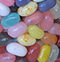
\includegraphics[width=\textwidth]{fig/img3}
      \caption{Unaltered.}
  \end{subfigure}
   \begin{subfigure}[b]{0.3\textwidth}
      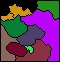
\includegraphics[width=\textwidth]{fig/wshed3}
      \caption{Watershed.}
  \end{subfigure}
   \begin{subfigure}[b]{0.3\textwidth}
      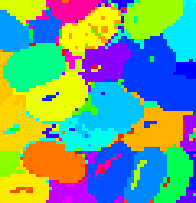
\includegraphics[width=\textwidth]{fig/ms3}
      \caption{Mean-shift.}
  \end{subfigure}
  \caption{Unaltered photo (a). Watershed (b) and mean shift (c) segmentation results. Different colors represent different clusters. (The black lines in the watershed picture are for clarity; they are omitted in the mean-shift picture due to the number of small clusters.)}
  \label{fig:unalt}
  \end{figure}

\section{Conclusion}

\section{References}

\end{document}